\section{Method}

In this section, we discuss our system design thoroughly. Fig.\ref{fig:system} shows the architecture of our system. The Pre-process Module and the Pre-process Table are actually shared by both scenario A and B, we take these together as an independent part, Preliminaries. And then Scenario A and B will be discussed separately.  

\begin{figure*}[htbp]
\centering {
	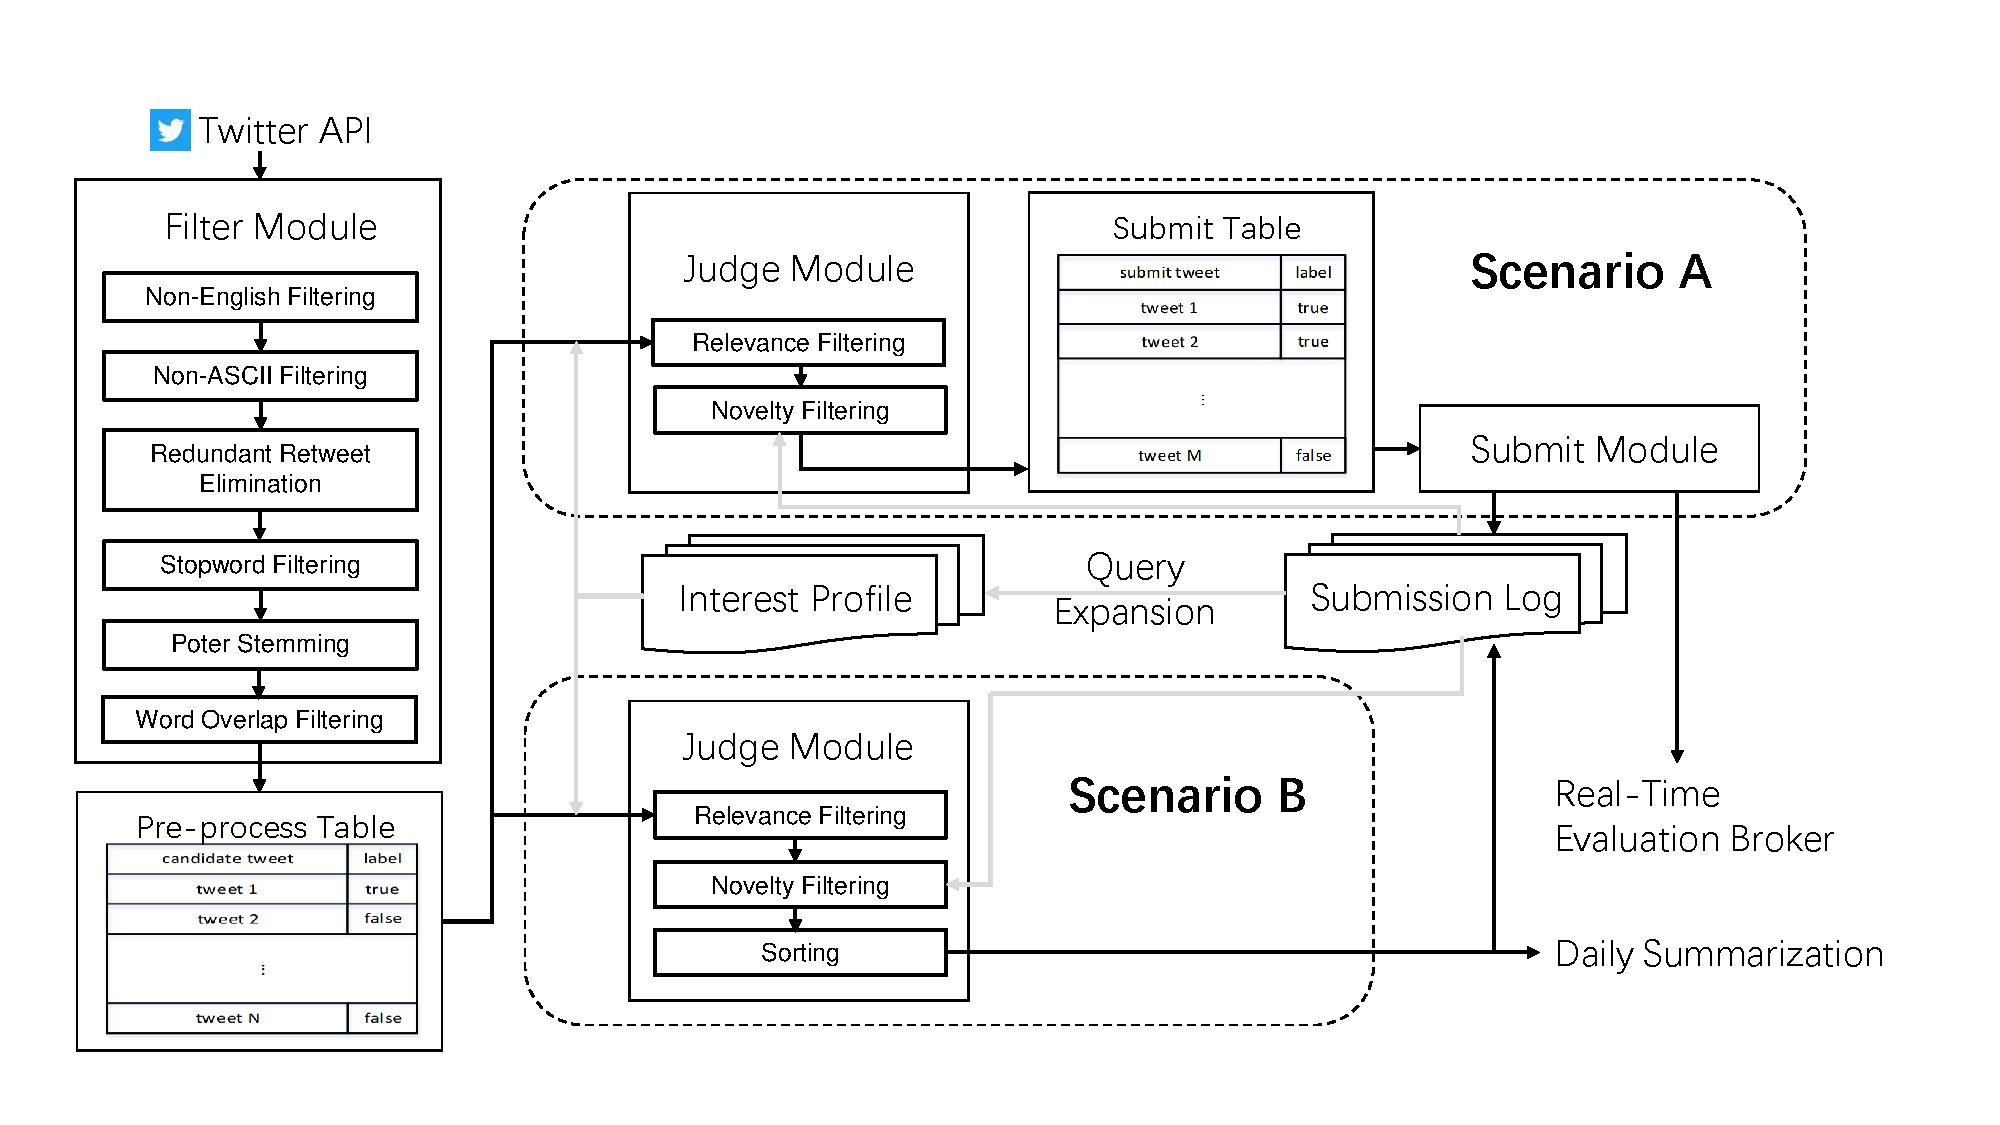
\epsfig{file=figures/system.pdf, width=\textwidth}
}
\caption{The System Architecture.}
\label{fig:system}
\end{figure*}

\subsection{Preliminaries}
In this section, we mainly talk about how our system perform preliminary operation,
to make the follow-up filtering easier and more precise.

\subsubsection{Filter Module}
The preprocessing we adopt on interest profile and tweet stream follows \cite{yao2016pkuicst} and \cite{lvpkuicst},
which is described as follows:

\begin{itemize}
\item \textbf{Non-English Filtering:}
Tweets written in a language other than English would be judged as not relevant
based on guidelines of Real-Time Summarization Track.
Thus, we use the twitter's language detector to abandon the non-English tweets.
\item \textbf{Non-ASCII Words:}
Removing all NON-ASCII characters from the tweets will also helps remove non-English tweets.
\item \textbf{Redundant Retweet Elimination:}
All additional commentary in the tweets containing ``RT @'' will be ignored.
As the guideline mentioned, all retweets should be normalized to the underlying tweets.
\item \textbf{Porter Stemming and Stopword Filtering:}
We remove all stopwords and stem the tweet text using the Natural Language Toolkit.
\item \textbf{Word Overlap Filtering:}
We filter out tweets that have no overlap with all interest profile in word-level,
because our methods don't consider semantic information. 
This can accelerate the he speed of identifying possible relevant tweets for each profile.
\end{itemize}

\subsubsection{Statistics Information}
In the language model, if any word in the query is not in the document,
the relevant score between them will equal to zero, which is unreasonable.
Smooth techniques could solve this problem by merging global word
probability distribution with current document model.
In our proposed approach, we obtain the global word probability distribution
by computing word count information of tweet stream during the 10 days before the evaluation period.

\subsection{Scenario A}
In this section, we will introduce our method for Scenario A.

\begin{itemize}
\item \textbf{Judge Module}
This module keeps 'listening' to the Pre-process Table. 
Every time a new inserted tweet is detected
(actually we collect a bunch of tweets in every time interval T1 in practice), 
that tweet is sent to the next stage for filtering. 
In the first stage of filtering, for every interest profile, we compute a relevance score 
using a text similarity function $f$. 
If that relevance score is bigger than the relevance threshold $\alpha$, 
this tweet-profile pair can go to the next stage.
In the second stage of filtering, for every selected tweet-profile pair, 
The same as previous stage, 
we compute the similarities using $f$ between the tweet and each of the pushed tweets of this profile,
we select the biggest one as the novelty score and compared to the novelty threshold $\beta$.
If that novelty score is smaller than $\beta$, 
we insert this tweet to the Submit Table, and remove it from the Pre-process Table.  
\item \textbf{Submit Module}
Like the Judge Module, this module keeps 'listening' to the Submit Table.
Every time a new inserted tweet is detected
(actually we collect a bunch of tweets in every time interval T2 in practice), 
that tweet is sent to the Evaluation Broker. 
If the response tell us the submission is accepted successfully,
we remove that tweet from the Submit Table and write it into the Submission Log.
Otherwise that tweet will stay in the Submit Table until a successful submission. 
\end{itemize} 


\subsubsection{Similarity Algorithm}

The key components of the Judge Module is the similarity function $f$.
We use $f$ to compute the similarity of (tweet, profile) pairs and (tweet, tweet) pairs.
Note that we only use the 'title' of each interest profile for computing similarities.
 
We utilize two different methods to model similarity.

\begin{itemize}
\item \textbf{negative KL-divergence language model}
One of the most powerful approach is language model. 
Each tweet $D$ and each interest profile $Q$ can be regard as a probability distribution.
We use notation $\widehat{\theta}_D$ and $\widehat{\theta}_Q$ to represent the language model respectively.
The negative KL-divergence between $\widehat{\theta}_Q$ and $\widehat{\theta}_D$ with the help of
collection language model $\widehat{\theta}_C$ can be calculated as below:

\begin{equation}
\begin{aligned}
DIR(Q,&D,C) = \sum_{w \in Q} P(w|\widehat{\theta}_Q) \cdot \\
&log \left( (1-\lambda) * P(w|\widehat{\theta}_D) + \lambda * P(w|\widehat{\theta}_C) \right), \\
with\; \lambda &= \frac{\mu}{|D| + \mu}
\end{aligned}
\end{equation}

\item \textbf{cosine distance}
Another method is using cosine distance model the similarity directly.
We build the IDF(Inverse Document Frequency) vector for each tweet and interest profile.
The IDF of each word is computed by the tweets collected before evaluation period,
as we have talked in the Preliminaries section.
The formula is shown below:

\begin{equation}
COS(Q,D) = \frac{\vec{Q} \cdot \vec{D}}{|\vec{Q}||\vec{D}|}
\end{equation}

\end{itemize}

\subsubsection{Query Expansion}

As microblog retrieval suffers severely from the vocabulary mismatch problem 
(i.e. term overlap between query and tweet is relatively small).
Query Expansion \cite{zhai2011mbfb} can play an important role in this situation. 
Moreover, more terms in the query makes retrieval more precise in general.

We use Pseudo Relevance Feedback technique to expand the interest profile 
with IDF-cosine method in PKUICSTRunA3 and PKUICSTRunB3.
At the end of each day, we collect the submitted tweets of each interest profile,
compute the word count, and sort by the word count.
For each interest profile, we add the top $K$ words that are not original in the profile to the profile.
We set the expanded words a weight $\gamma (\gamma < 1)$ while the original words with a default weight 1.  

\subsubsection{Parameter Selection}

The parameters shown in Table.\ref{tab:paraA} are tuned via grid search on TREC 2016 dataset.

\begin{table}[htbp]
\newcommand{\tabincell}[2]{\begin{tabular}{@{}#1@{}}#2\end{tabular}}
\centering
\caption{Parameters of the Push Notifications Scenario.}
\label{tab:paraA}
\begin{tabular}{lcccc}
\hline
Run ID&$f$&$\alpha$&$\beta$&\tabincell{c}{Query\\Expansion}\\
\hline
PKUICSTRunA1&\tabincell{c}{DIR\\$\mu=50$}&0.7&0.5&-\\
PKUICSTRunA2&COS&0.8&0.85&-\\
PKUICSTRunA3&COS&0.8&0.85&\tabincell{c}{$K=2$\\$\gamma=0.2$}\\
\hline
\end{tabular}
\end{table}

\subsection{Scenario B}

From Figure.\ref{fig:system}, we can see our approach of Scenario B is not much different from that of Scenario A.
We remove the Submit Module and Submit Table, and add a sorting process at the end of Judge Module.
Besides, we try to utilize model blending in this scenario.
Model blending has been proved useful in many situation.
We simply use the formula below to blend our two similarity models discussed before.

\begin{equation}
\begin{aligned}
BL(Q,D,C) = &\delta \cdot DIR(Q,D,C)+ \\
&(1-\delta)\cdot COS(Q,D), 0 < \delta < 1
\end{aligned}
\end{equation}   

\subsubsection{Parameter Selection}

Like Scenario A, these parameters shown in Table.\ref{tab:paraB} are tuned via grid search on TREC 2016 dataset.

\begin{table}[htbp]
\newcommand{\tabincell}[2]{\begin{tabular}{@{}#1@{}}#2\end{tabular}}
\centering
\caption{Parameters of the Push Notifications Scenario.}
\label{tab:paraB}
\begin{tabular}{lcccc}
\hline
Run ID&$f$&$\alpha$&$\beta$&\tabincell{c}{Query\\Expansion}\\
\hline
PKUICSTRunB1&\tabincell{c}{DIR\\$\mu=50$}&0.72&0.72&-\\
PKUICSTRunB2&\tabincell{c}{BL\\$\mu=50$ \\ $\delta=0.5$ }&0.78&0.78&-\\
PKUICSTRunB3&\tabincell{c}{BL\\$\mu=50$ \\ $\delta=0.5$}&0.78&0.78&\tabincell{c}{$K=2$\\$\gamma=0.2$}\\
\hline
\end{tabular}
\end{table}
